\section{\scshape Best views estimation}
\subsection*{Best views estimation}

\begin{frame}{Reference surface point cloud}
	\begin{itemize}
		\item The first step in the processing pipeline includes the generation of the multi-object reference point cloud that is assembled using the CAD data and the objects poses given by the simulator, which is later on filtered with a voxel grid algorithm to perform a regular spatial partition and extract the points that are in the surface voxels centroids
	\end{itemize}
	\begin{figure}
		\centering
		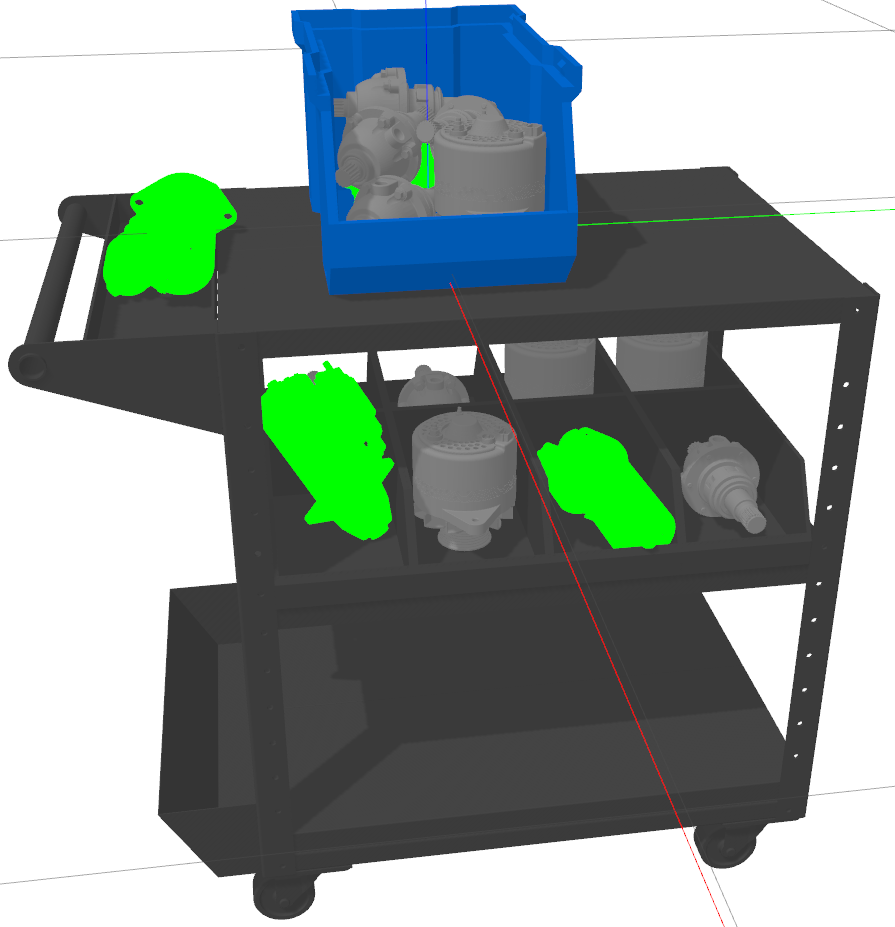
\includegraphics[height=.27\textheight]{sensor-data-processing/multimodel-environment}
		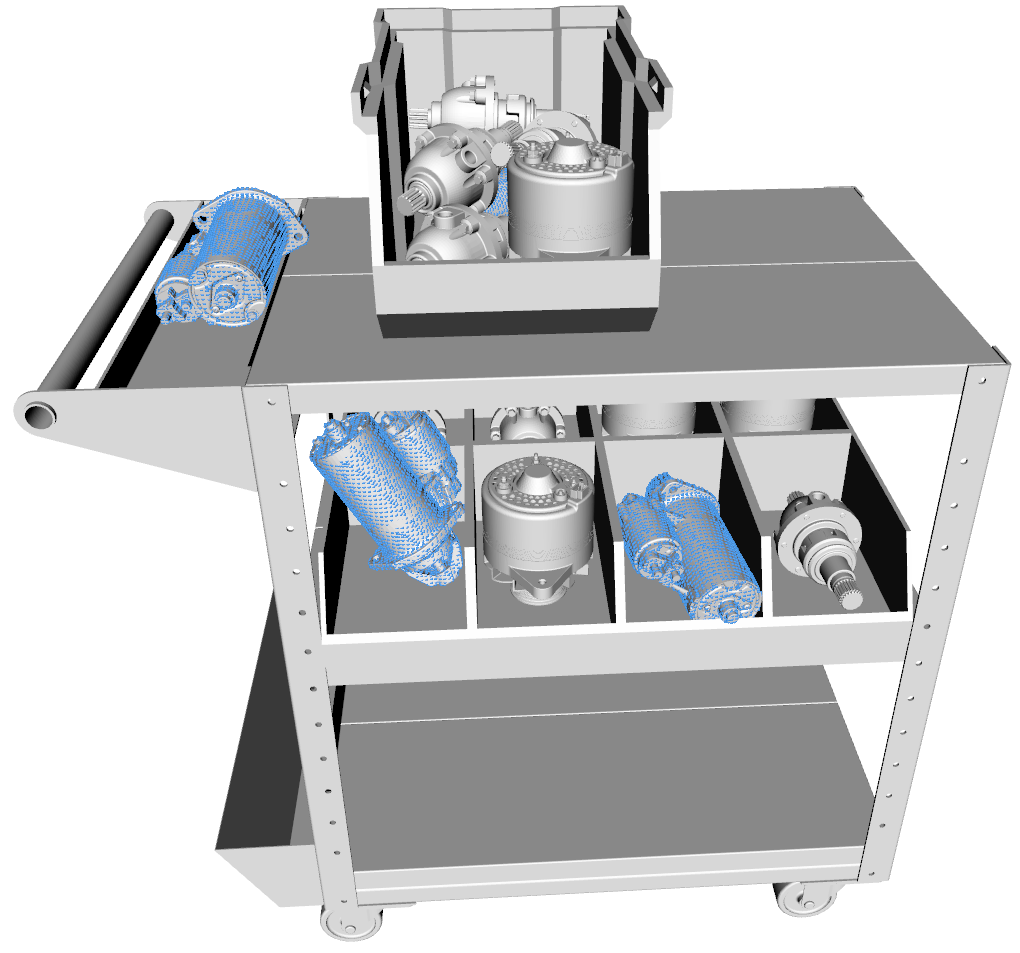
\includegraphics[height=.27\textheight]{sensor-data-processing/multimodel-pointclouds-with-cad}
		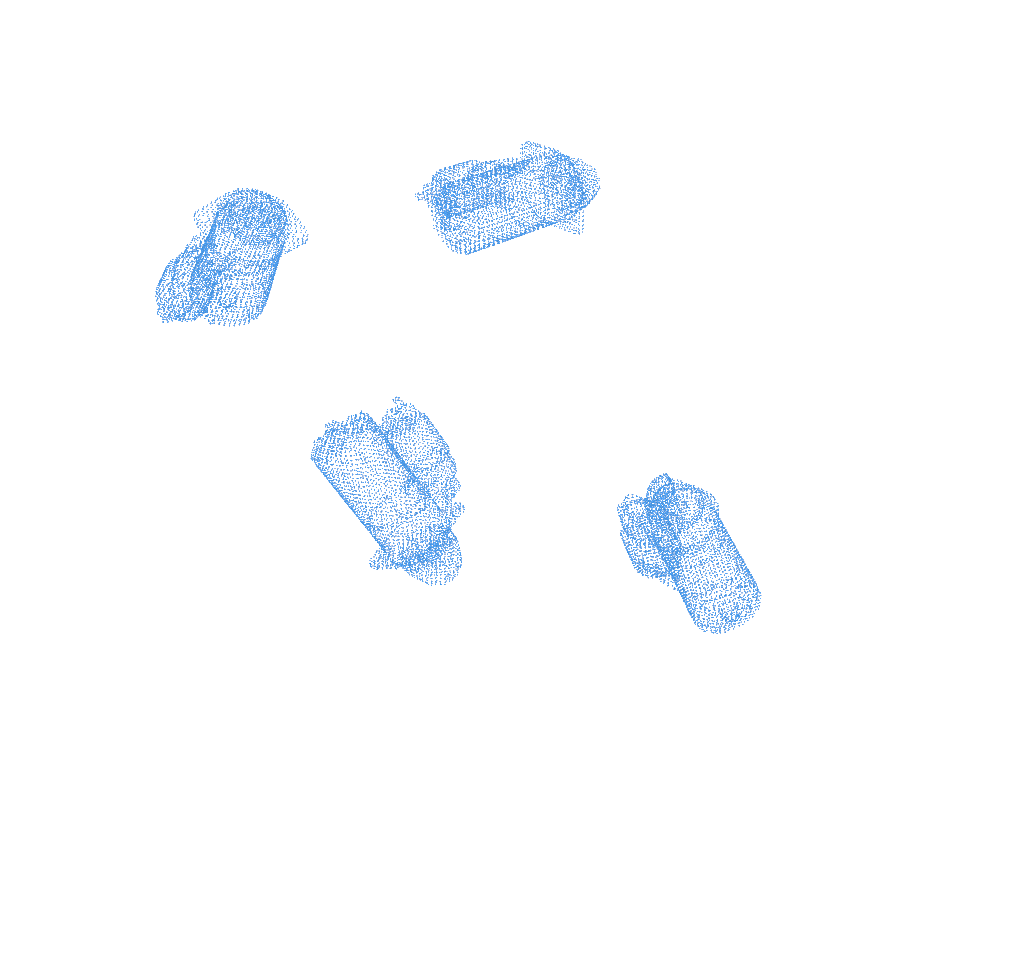
\includegraphics[height=.27\textheight]{sensor-data-processing/multimodel-pointclouds}
		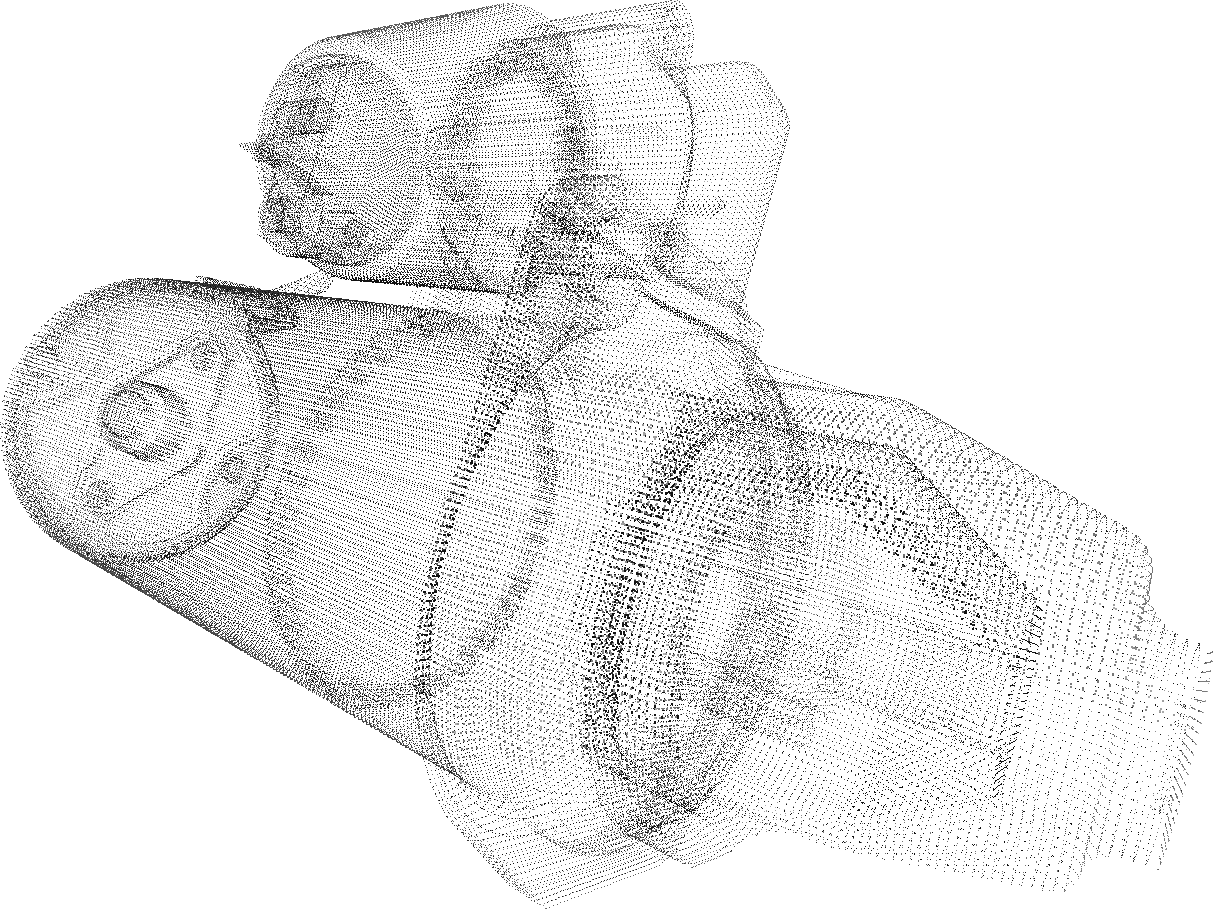
\includegraphics[height=.27\textheight]{sensor-data-processing/cad-model-pointcloud}
		\caption{The first image illustrates the color scene rendering in Gazebo with the target objects in green while the second and third images display the reference point cloud that was generated from the CAD points data shown on the last image}
	\end{figure}
\end{frame}

\begin{frame}{Sensors data analysis}
	\begin{itemize}
		\item Given a set of deployed sensors in the simulation world, for each sensor it is computed the voxelized point cloud of the observed target object(s) points:
		\begin{itemize}
			\item Color segmentation is performed to identify the sensor image pixels that belong to the target object(s) (which have a unique pure green material)
			\item For each image pixel associated with a target object, the 3D depth point is computed from the z-buffer depth image using the pinhole camera model
			\item The generated point cloud is transformed from the sensor into the world coordinate system frame
			\begin{itemize}
				\item Allows fast merging of point clouds generated from different sensors
			\end{itemize}
			\item A voxel grid filtering algorithm is applied to perform a regular space partition in which the points centroid are computed for each voxel
			\begin{itemize}
				\item Critical for allowing consistent evaluation of the object(s) observed surface percentage, even when the sensors have different resolution and are at different distances from the target object(s)
			\end{itemize}
		\end{itemize}
	\end{itemize}
\end{frame}


\begin{frame}{Sensors data analysis}
	\begin{figure}
		\centering
		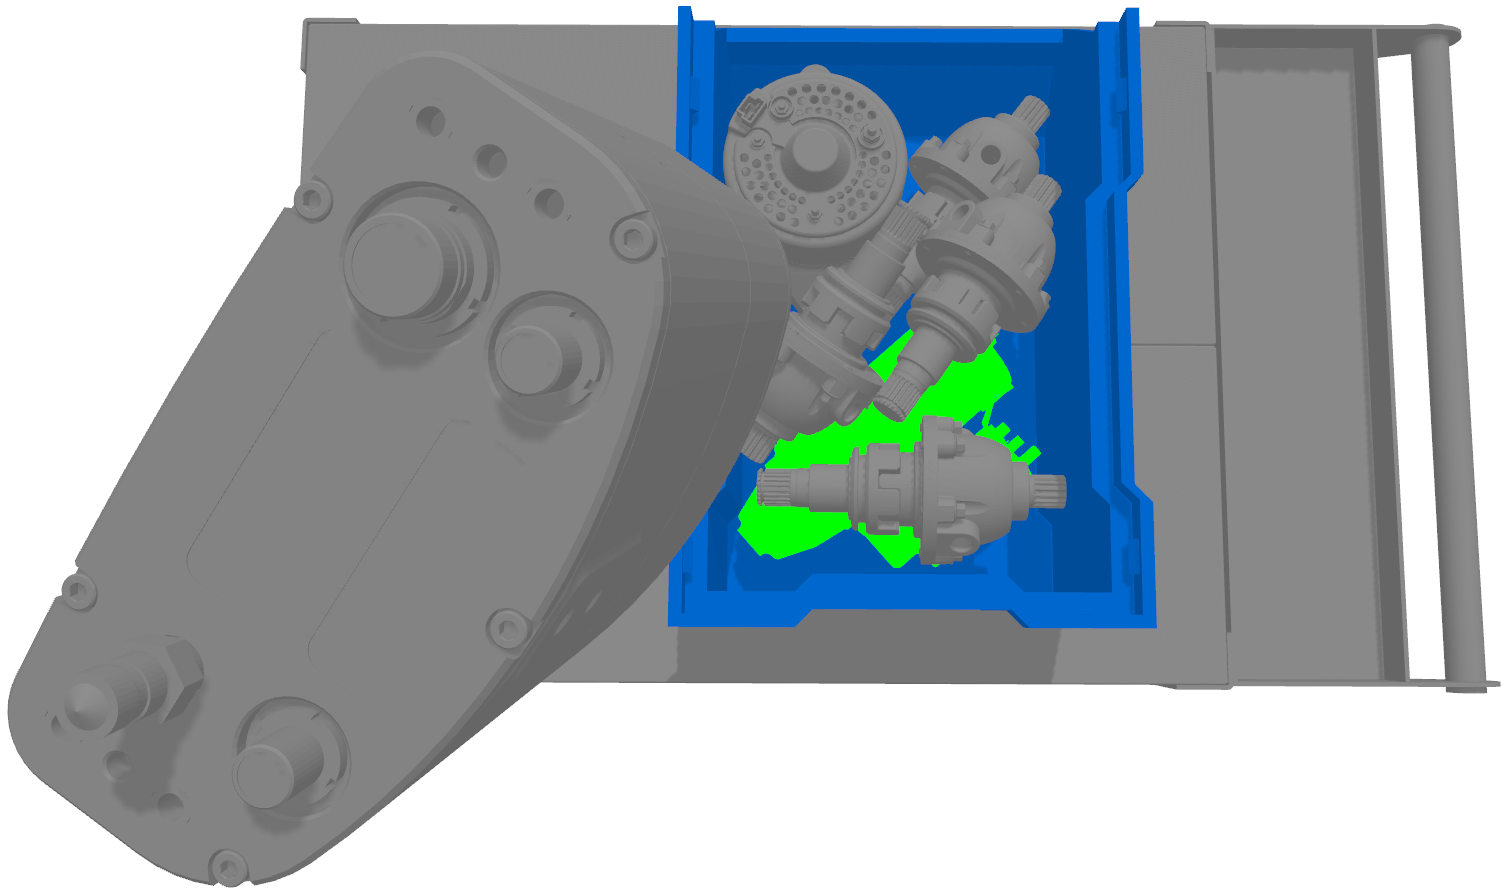
\includegraphics[height=.32\textheight]{sensor-data-processing/sensors-best-view}\\
		\vspace{0.5em}
		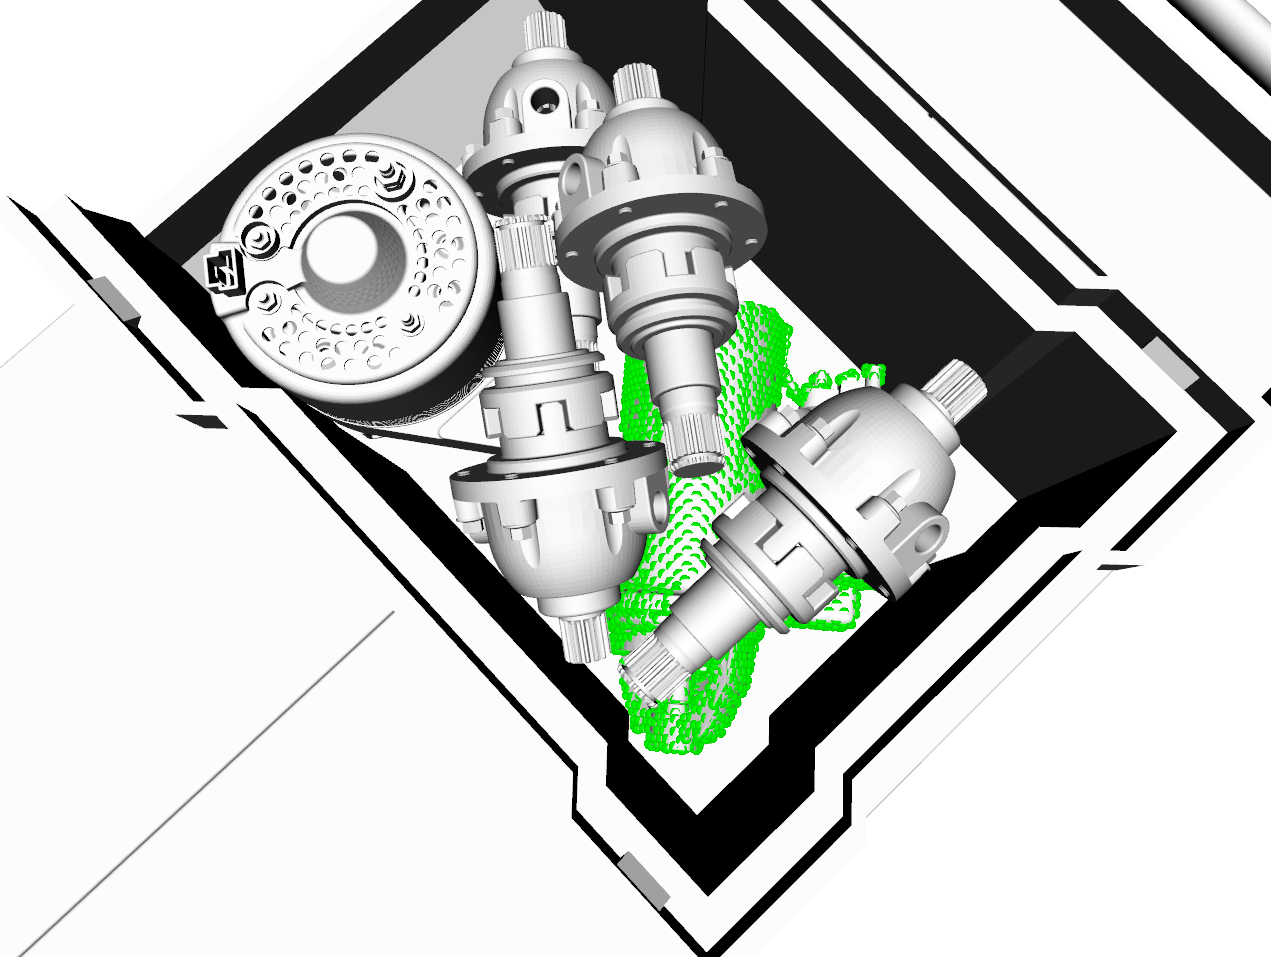
\includegraphics[height=.32\textheight]{sensor-data-processing/rviz-sensor-view}\hspace{2em}
		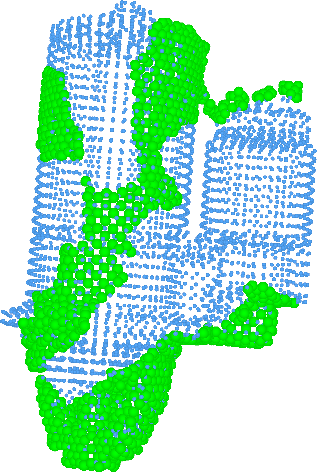
\includegraphics[height=.32\textheight]{sensor-data-processing/rviz-sensor-view-without-cad-with-model}
		\caption{Color image rendered with the gazebo simulator (top image containing the scene and sensor) along with the generated point cloud for the target object taking into consideration the environment occlusions (bottom images, in which the green spheres are the observed points and the blue spheres are from the point cloud of the associated CAD model)}
	\end{figure}
\end{frame}


\begin{frame}{Estimation of the best sensor}
	After having the processed point cloud for each deployed sensor:
	\begin{itemize}
		\item If only one sensor is enough (decision made by the system user):
		\begin{itemize}
			\item The surface coverage percentage for each sensor is computed
			\begin{itemize}
				\item Given that both the reference point cloud and sensor data were filtered with a voxel grid with the same resolution and in the same coordinate system frame, calculating the surface coverage percentage can be efficiently computed by simply dividing the number of surface voxel points in the sensor data by the number of surface voxel points in the reference point cloud
			\end{itemize}
			\item The sensor that can observe the most surface area percentage of the target object(s) is chosen
		\end{itemize}
	\end{itemize}
\end{frame}


\begin{frame}{Estimation of the best N sensors disposition}
	After having the processed point cloud for each deployed sensor:
	\begin{itemize}
		\item If several sensors can be used (decision made by the system user):
		\begin{itemize}
			\item Using a Random Sample Consensus (RANSAC) approach, a set of N sensors is chosen randomly
			\item The sensor data from the selected sensors is merged
			\item The voxel grid filter algorithm is applied to ensure that there is only one point per voxel
			\item The observable surface area percentage for the selected sensors is computed
			\item If current subset of sensors achieved better observable surface area percentage than the current best, then it becomes the current best views estimation for the sensor disposition
			\item At the end of a given number of iterations or if the observable surface area percentage reaches a given threshold, the search is terminated, returning the best sensor configuration found
		\end{itemize}
	\end{itemize}
\end{frame}


\begin{frame}{Active perception environment - 1 sensor}
	\begin{figure}
		\centering
		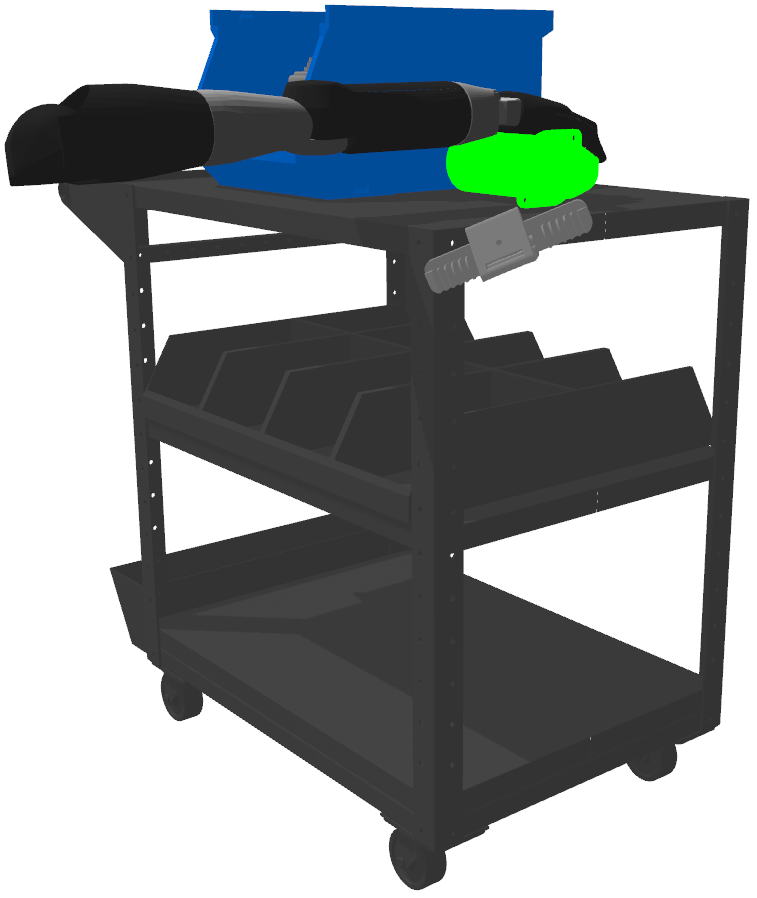
\includegraphics[height=.26\textwidth]{best-views-estimation/active-perception/1-sensor/gazebo-corner}\hspace{4em}
		\includegraphics[height=.26\textwidth]{best-views-estimation/active-perception/1-sensor/rviz-front-corner}\\
		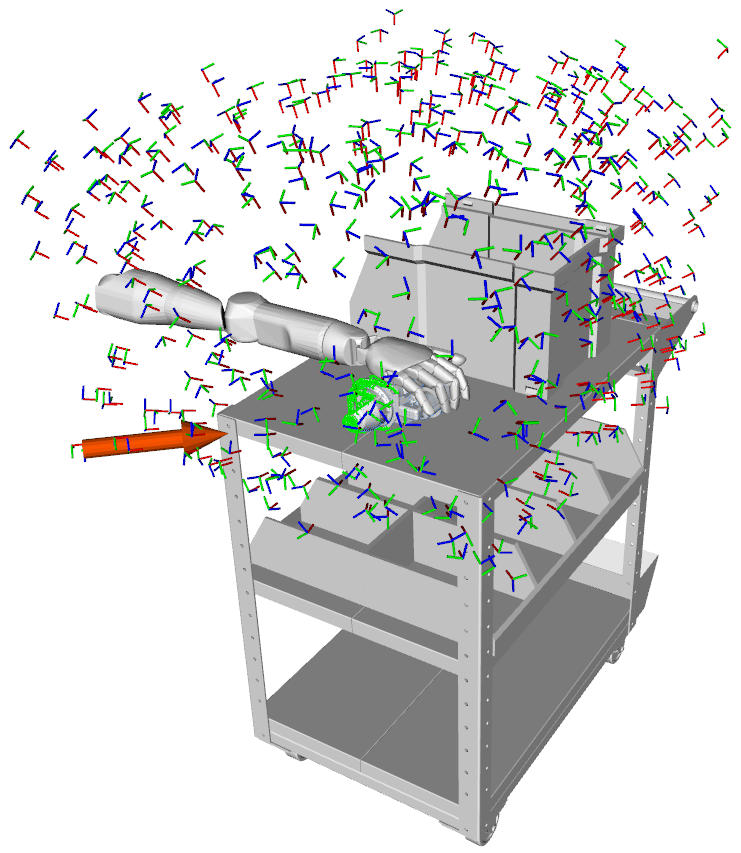
\includegraphics[height=.26\textwidth]{best-views-estimation/active-perception/1-sensor/rviz-back-corner}\hspace{2em}
		\includegraphics[height=.26\textwidth]{best-views-estimation/active-perception/1-sensor/rviz-top}
		\caption{Estimation of the best sensor position for the active perception environment with a 27.73\% of surface area coverage (top left showing the Gazebo color rendering and remaining images displaying the best sensor as a large red arrow, the deployed sensors as small coordinate frames and the observed sensor data as green spheres)}
	\end{figure}
\end{frame}


\begin{frame}{Active perception environment - 3 sensors}
	\begin{figure}
		\centering
		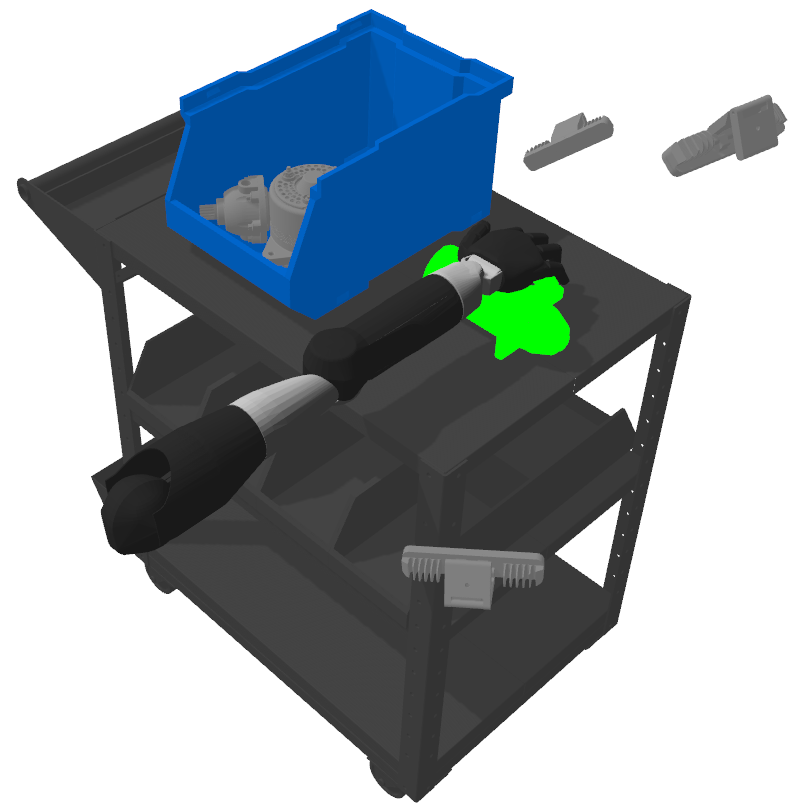
\includegraphics[height=.32\textwidth]{best-views-estimation/active-perception/3-sensors/gazebo-front-right-corner}\hspace{4em}
		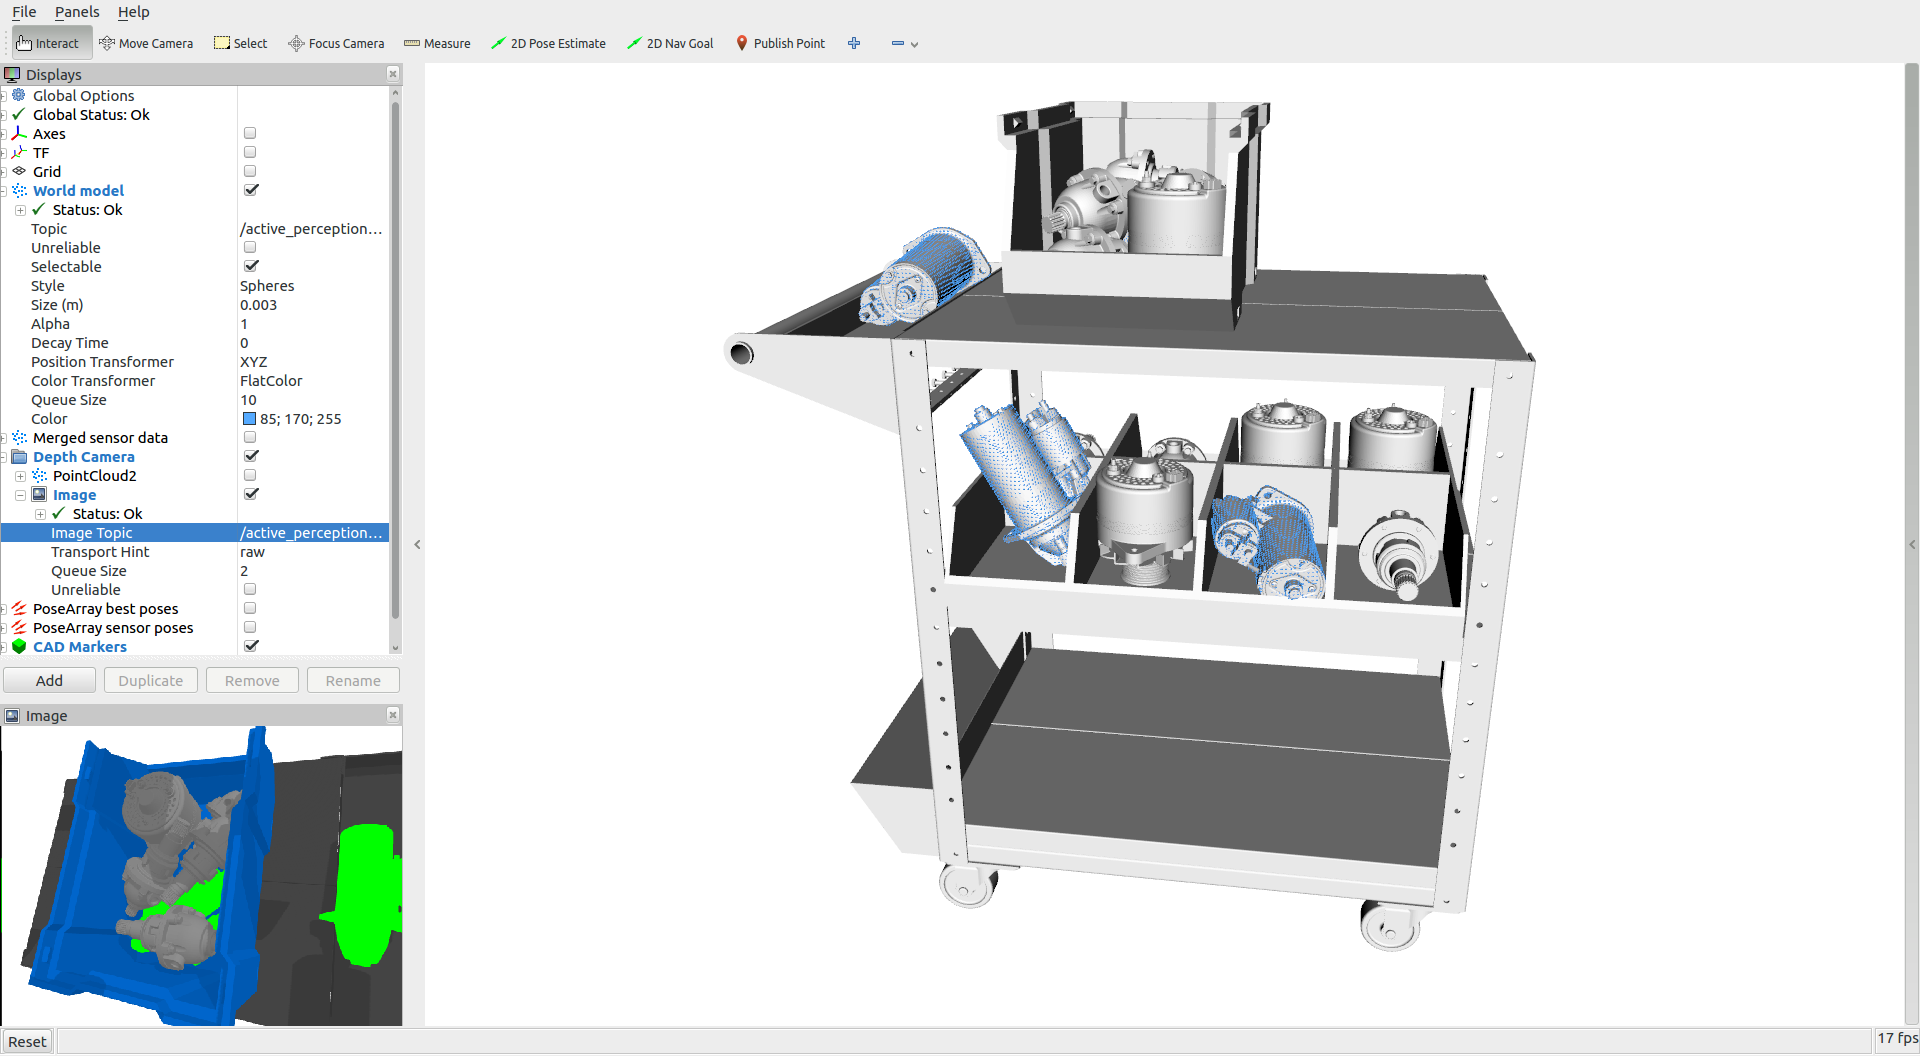
\includegraphics[height=.32\textwidth]{best-views-estimation/active-perception/3-sensors/rviz-front-right}\\
		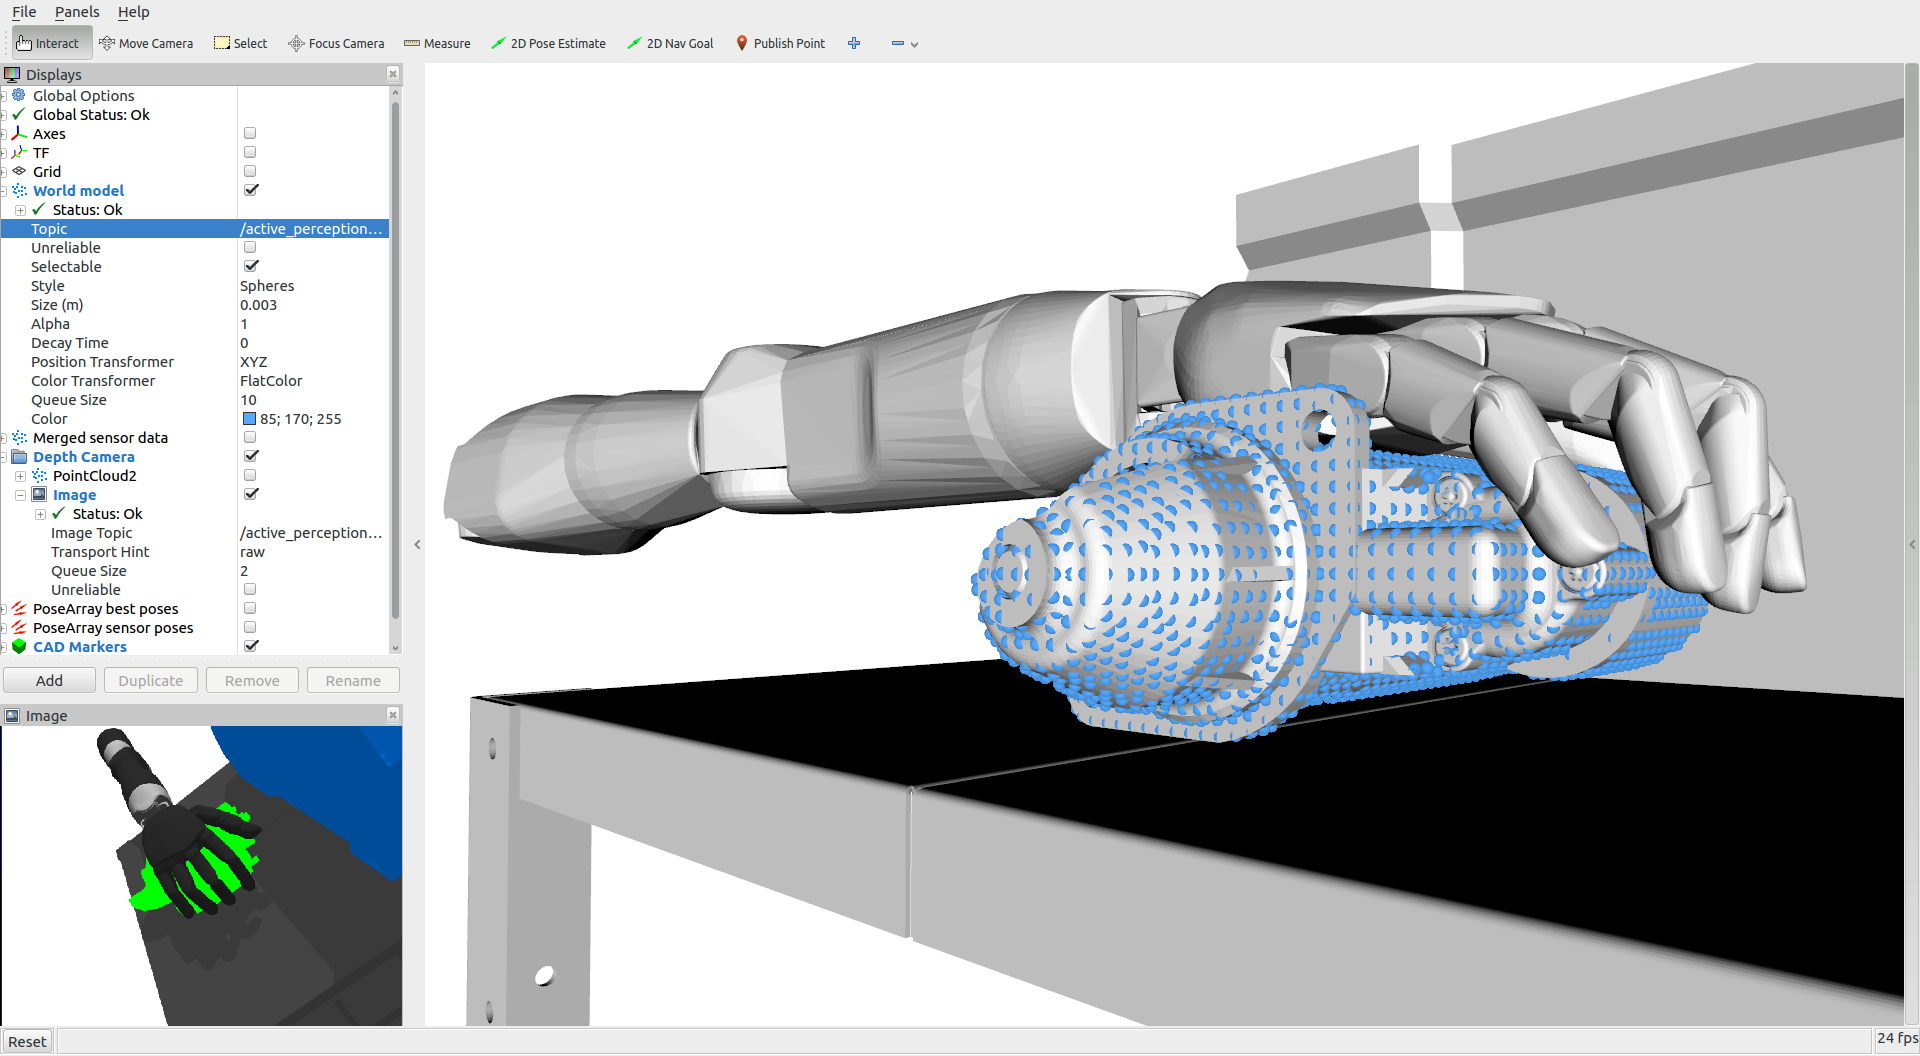
\includegraphics[height=.32\textwidth]{best-views-estimation/active-perception/3-sensors/rviz-back-left}\hspace{2em}
		\includegraphics[height=.32\textwidth]{best-views-estimation/active-perception/3-sensors/rviz-top}
		\caption{Estimation of the best 3 sensors disposition for the active perception environment with a 61.91\% of surface area coverage}
	\end{figure}
\end{frame}


\begin{frame}{Bin picking environment - 1 sensor}
	\begin{figure}
		\centering
		\includegraphics[height=.27\textwidth]{best-views-estimation/bin-picking/1-sensor/gazebo-top}\hspace{2em}
		\includegraphics[height=.27\textwidth]{best-views-estimation/bin-picking/1-sensor/rviz-front}\\
		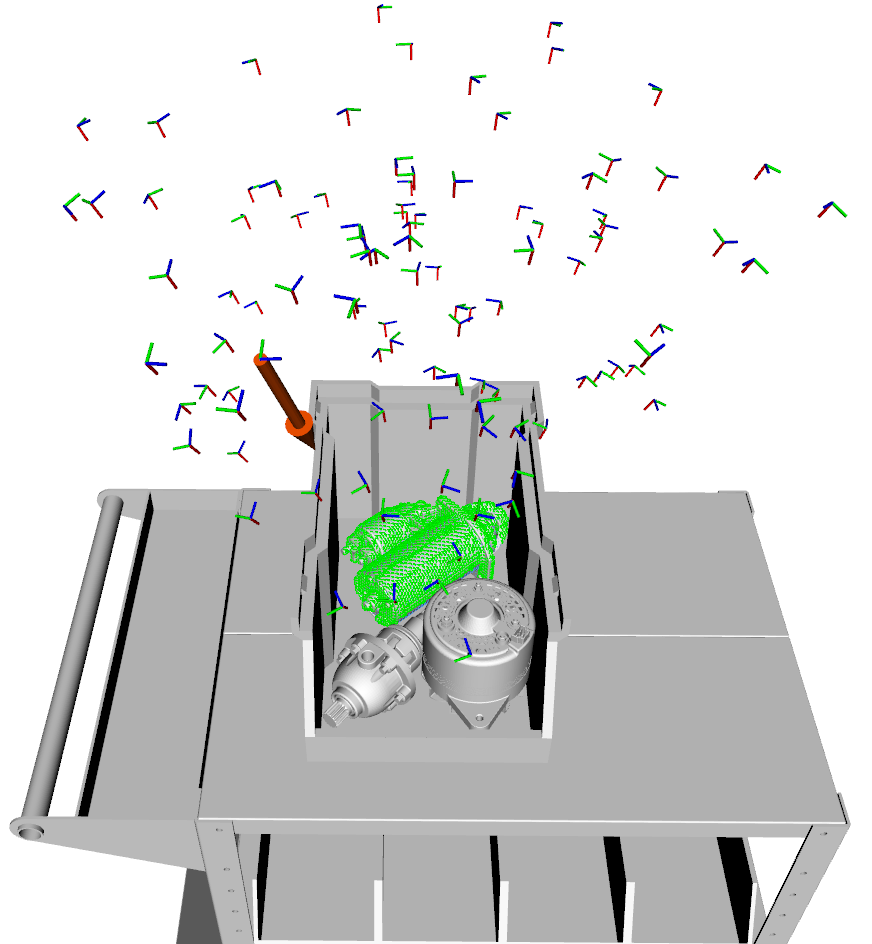
\includegraphics[height=.35\textwidth]{best-views-estimation/bin-picking/1-sensor/rviz-top-front}\hspace{4em}
		\includegraphics[height=.35\textwidth]{best-views-estimation/bin-picking/1-sensor/rviz-top}
		\caption{Estimation of the best sensor position for the bin picking environment with a 45.10\% of surface area coverage}
	\end{figure}
\end{frame}


\begin{frame}{Bin picking environment - 5 sensors}
	\begin{figure}
		\centering
		\includegraphics[height=.3\textwidth]{best-views-estimation/bin-picking/5-sensors/gazebo-front}\hspace{2em}
		\includegraphics[height=.3\textwidth]{best-views-estimation/bin-picking/5-sensors/rviz-top}\\
		\includegraphics[height=.3\textwidth]{best-views-estimation/bin-picking/5-sensors/rviz-corner}\hspace{2em}
		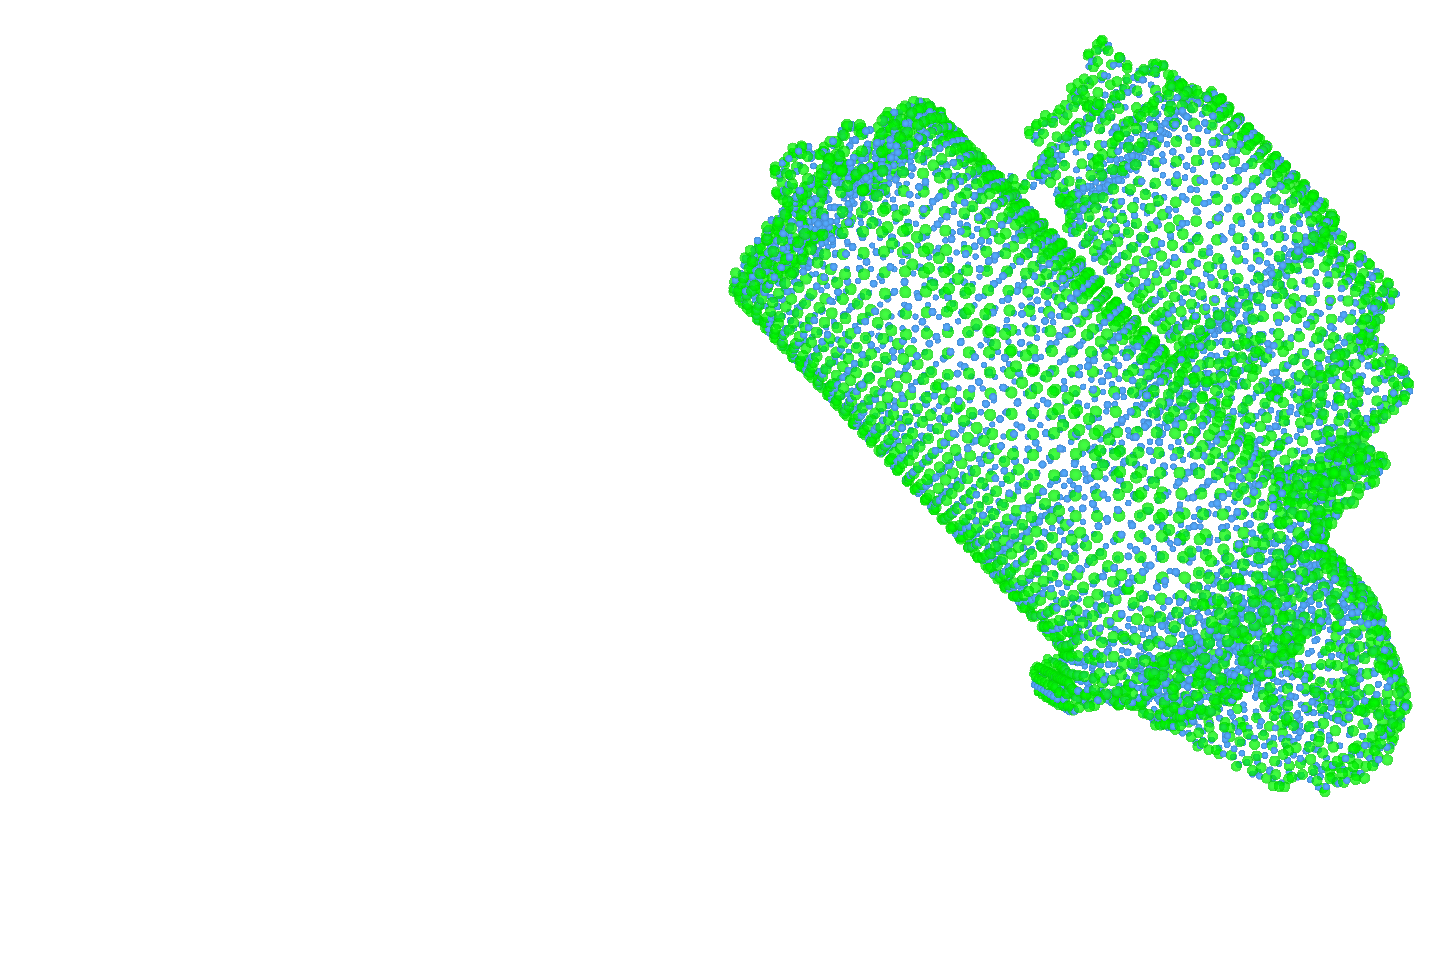
\includegraphics[height=.3\textwidth]{best-views-estimation/bin-picking/5-sensors/rviz-sensor-data}
		\caption{Estimation of the best 5 sensors disposition for the bin picking environment with a 64.63\% of surface area coverage}
	\end{figure}
\end{frame}


\begin{frame}{Bin picking with occlusions environment - 1 sensor}
	\begin{figure}
		\centering
		\includegraphics[height=.28\textwidth]{best-views-estimation/bin-picking-with-occlusions/1-sensor/gazebo-top}\hspace{2em}
		\includegraphics[height=.28\textwidth]{best-views-estimation/bin-picking-with-occlusions/1-sensor/rviz-corner}\\
		\includegraphics[height=.28\textwidth]{best-views-estimation/bin-picking-with-occlusions/1-sensor/rviz-front}\hspace{4em}
		\includegraphics[height=.28\textwidth]{best-views-estimation/bin-picking-with-occlusions/1-sensor/rviz-top}
		\caption{Estimation of the best sensor position for the bin picking with occlusions environment with a 19.27\% of surface area coverage}
	\end{figure}
\end{frame}


\begin{frame}{Bin picking with occlusions environment - 3 sensors}
	\begin{figure}
		\centering
		\includegraphics[height=.28\textwidth]{best-views-estimation/bin-picking-with-occlusions/3-sensors/gazebo-top}\hspace{2em}
		\includegraphics[height=.28\textwidth]{best-views-estimation/bin-picking-with-occlusions/3-sensors/rviz-front}\\
		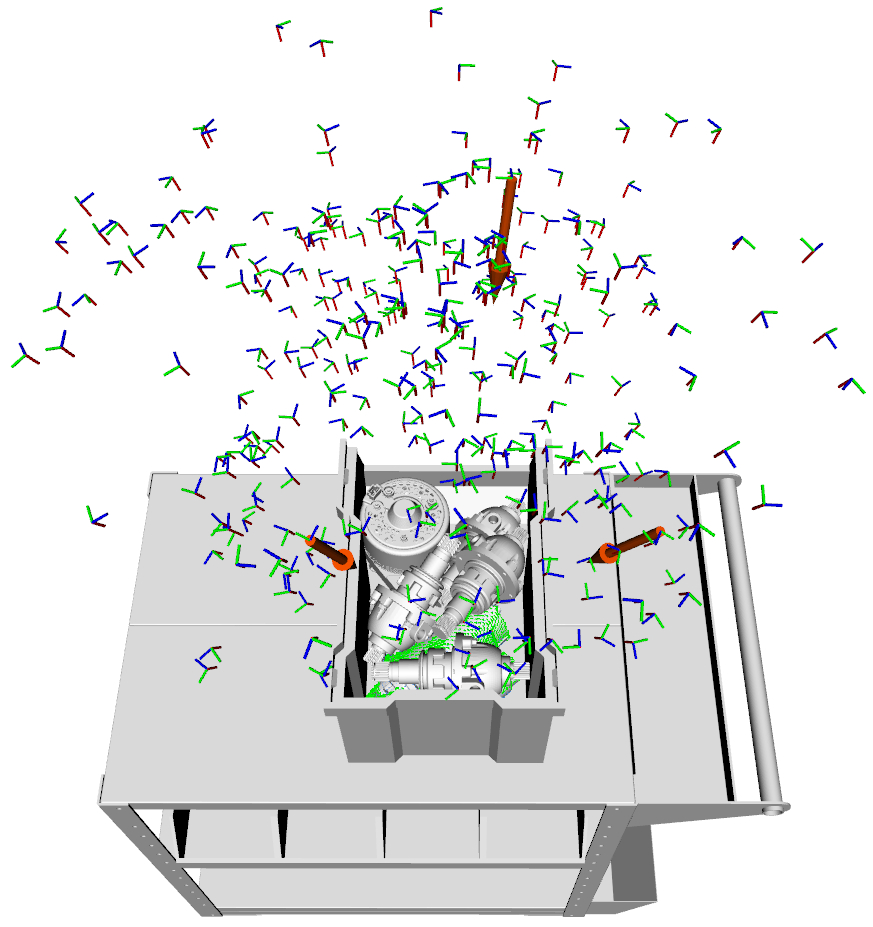
\includegraphics[height=.28\textwidth]{best-views-estimation/bin-picking-with-occlusions/3-sensors/rviz-top-back}\hspace{4em}
		\includegraphics[height=.28\textwidth]{best-views-estimation/bin-picking-with-occlusions/3-sensors/rviz-top}
		\caption{Estimation of the best 3 sensors disposition for the bin picking with occlusions environment with a 31.19\% of surface area coverage}
	\end{figure}
\end{frame}


\begin{frame}{Multiple bin picking with occlusions environment - 10 sensors}
	\begin{figure}
		\centering
		\includegraphics[height=.28\textwidth]{best-views-estimation/multiple-bin-picking-with-occlusions/10-sensors/gazebo-front}\hspace{2em}
		\includegraphics[height=.28\textwidth]{best-views-estimation/multiple-bin-picking-with-occlusions/10-sensors/rviz-front-corner}\\
		\includegraphics[height=.28\textwidth]{best-views-estimation/multiple-bin-picking-with-occlusions/10-sensors/rviz-front}\hspace{1.5em}
		\includegraphics[height=.28\textwidth]{best-views-estimation/multiple-bin-picking-with-occlusions/10-sensors/rviz-top}
		\caption{Estimation of the best 10 sensors disposition for the multiple bin picking with occlusions environment with a 43.93\% of surface area coverage}
	\end{figure}
\end{frame}
